% chip-quantum-catalog.tex
% Quantum redefinition of stack, queue, and cosine similarity
% on the complex Cartesian plane — with Dirac, Einstein, Knuth,
% code tables AAAA...FFFFF, and the BubbleLeader builder chain.
%
% Compile: pdflatex chip-quantum-catalog.tex
% Grammar: docs/xml/chip-queries.xml (lang=XML.g())
% Python:  singine-collibra/python/singine_collibra/quantum_catalog.py
% Collibra: cosine().similarity().complex().resolve().xml().catalog().collibra()

\documentclass[12pt,a4paper]{article}

\usepackage[utf8]{inputenc}
\usepackage[T1]{fontenc}
\usepackage{amsmath, amssymb, amsthm}
\usepackage{mathtools}
\usepackage{physics}          % \ket{}, \bra{}, \braket{}, \comm{}{}
\usepackage{tensor}
\usepackage{tikz}
\usepackage{pgfplots}
\pgfplotsset{compat=1.18}
\usetikzlibrary{angles, quotes, arrows.meta, decorations.pathreplacing, calc}
\usepackage{xcolor}
\usepackage{listings}
\usepackage{hyperref}
\usepackage{geometry}
\usepackage{booktabs}
\usepackage{array}
\usepackage{multicol}

\geometry{margin=2.5cm}

\definecolor{collibraBlue}{HTML}{0057B8}
\definecolor{quantumViolet}{HTML}{7B2FBE}
\definecolor{godelGray}{HTML}{4A4A4A}
\definecolor{escherGold}{HTML}{C8A400}
\definecolor{pgGreen}{HTML}{336791}

\lstset{
  basicstyle=\ttfamily\footnotesize,
  keywordstyle=\color{collibraBlue}\bfseries,
  commentstyle=\color{godelGray}\itshape,
  stringstyle=\color{quantumViolet},
  breaklines=true,
  frame=single,
  rulecolor=\color{gray!40},
}

\newtheorem{defn}{Definition}
\newtheorem{thm}{Theorem}
\newtheorem{axiom}{Axiom}

% ── Custom operators ─────────────────────────────────────────────────────────
\DeclareMathOperator{\Push}{\widehat{P}^\dagger}
\DeclareMathOperator{\Pop}{\widehat{P}}
\DeclareMathOperator{\Enq}{\widehat{Q}^\dagger}
\DeclareMathOperator{\Deq}{\widehat{Q}}
\DeclareMathOperator{\cossim}{cos\_sim}
\DeclareMathOperator{\JD}{JD}
\DeclareMathOperator{\diracD}{\delta}
\newcommand{\gonum}[1]{\ulcorner #1 \urcorner}
\newcommand{\Ctable}[1]{\texttt{\textbf{#1}}}

% ── Title ─────────────────────────────────────────────────────────────────────
\title{%
  \textcolor{collibraBlue}{\Large Quantum Catalog}\\[0.4em]
  \large Stack, Queue, Cosine Similarity\\
  on the Complex Cartesian Plane\\[0.6em]
  \normalsize
  \texttt{dirac()} $\cdot$ \texttt{einstein()} $\cdot$ \texttt{knuth()} $\cdot$
  \texttt{tex()} $\cdot$ \texttt{latex()} $\cdot$ \texttt{jd()} $\cdot$
  \texttt{refData()} $\cdot$ \texttt{collibra().init()}\\[0.3em]
  \texttt{loadCodeTableFromBaseFromShiva()} $\cdot$
  \texttt{bubbleLeader().builder()}\ldots\texttt{.paulGraham()}\\[0.3em]
  \texttt{cosine().similarity().complex().resolve().xml().catalog().collibra()}
}
\author{Singine Collibra \texttt{chip-queries.xml} $\;\cdot\;$ \texttt{lang=XML.g()}}
\date{2026-03-26}

\begin{document}
\maketitle
\tableofcontents
\bigskip\hrule\bigskip

% ════════════════════════════════════════════════════════════════════════════
\section{\texttt{dirac()} — Quantum State Notation}
% ════════════════════════════════════════════════════════════════════════════

The Dirac delta distribution $\diracD(x)$ and bra-ket notation form the
primitive vocabulary of this catalog.

\begin{defn}[Dirac delta]
\[
  \diracD(x - x_0) = \lim_{\varepsilon \to 0}
    \frac{1}{\varepsilon\sqrt{\pi}}\, e^{-(x-x_0)^2/\varepsilon^2},
  \qquad
  \int_{-\infty}^{\infty} \diracD(x - x_0)\, f(x)\, \dd x = f(x_0)
\]
\end{defn}

\begin{defn}[Bra-ket]
A quantum state lives in Hilbert space $\mathcal{H}$.
Ket: $\ket{\psi} \in \mathcal{H}$.
Bra: $\bra{\phi} \in \mathcal{H}^*$.
Inner product: $\braket{\phi}{\psi} \in \mathbb{C}$.
Outer product (projection): $\ketbra{\psi}{\psi}$.
\end{defn}

Completeness relation:
\[
  \sum_n \ket{n}\bra{n} = \hat{\mathbf{1}}, \qquad
  \int \ket{x}\bra{x}\, \dd x = \hat{\mathbf{1}}
\]

% ════════════════════════════════════════════════════════════════════════════
\section{\texttt{einstein()} — Data Gravity Field Equations}
% ════════════════════════════════════════════════════════════════════════════

\subsection{General Relativity}

Einstein's field equations:
\[
  \boxed{G_{\mu\nu} + \Lambda g_{\mu\nu} = \frac{8\pi G}{c^4}\, T_{\mu\nu}}
\]
where $G_{\mu\nu} = R_{\mu\nu} - \tfrac{1}{2} R\, g_{\mu\nu}$ is the Einstein tensor,
$\Lambda$ the cosmological constant, $T_{\mu\nu}$ the stress-energy tensor.

Special relativity: $E = mc^2$, covariant form:
\[
  p^\mu p_\mu = \eta_{\mu\nu} p^\mu p^\nu = -\left(\frac{E}{c}\right)^2 + |\mathbf{p}|^2 c^2 = -(mc)^2
\]

\subsection{Data Gravity Analog}

For a data platform with usage tensor $T_{\mu\nu}^{\text{data}}$:
\[
  G_{\mu\nu}^{\text{info}} + \Lambda_{\text{latency}}\, g_{\mu\nu}
  = \frac{8\pi G_{\text{info}}}{c_{\text{latency}}^4}\, T_{\mu\nu}^{\text{usage}}
\]

The \emph{ultimate metric} (CLAUDE.md) maps to:
\[
  \mathcal{U} = \underbrace{\alpha\, U_{\text{usage}}}_{\text{usage volume}}
              + \underbrace{\beta\, V_{\text{business}}}_{\text{business value}}
              - \underbrace{\gamma\, C_{\text{platform}}}_{\text{platform cost}}
\]
Optimum: $\nabla_\theta \mathcal{U} = \mathbf{0}$, i.e.\ saddle-point of the
information Lagrangian $\mathcal{L} = \mathcal{U} - \lambda(\text{constraints})$.

% ════════════════════════════════════════════════════════════════════════════
\section{\texttt{knuth()} — Algorithmic Notation}
% ════════════════════════════════════════════════════════════════════════════

\subsection{Asymptotic notation (Knuth, TAOCP)}

\[
  f(n) = O(g(n)) \iff \exists\, c{>}0,\, n_0 : |f(n)| \leq c\,|g(n)|\ \forall n \geq n_0
\]
\[
  f(n) = \Omega(g(n)) \iff g(n) = O(f(n)), \qquad
  f(n) = \Theta(g(n)) \iff f{=}O(g) \land g{=}O(f)
\]

\subsection{Knuth up-arrow notation}

\[
  a \uparrow b = a^b, \quad
  a \uparrow\uparrow b = \underbrace{a^{a^{\iddots^a}}}_{b}, \quad
  a \uparrow\uparrow\uparrow b = \underbrace{a \uparrow\uparrow (a \uparrow\uparrow \cdots)}_{b}
\]

The BubbleLeader builder chain (§\ref{sec:bubble}) composes
$n = 13$ functions; its worst-case complexity:
\[
  T_{\text{chain}}(n) = \Theta\!\left(\sum_{k=1}^{13} T_k\right)
  = \Theta(n \log n) \text{ (dominated by sort in } \texttt{pg()}\text{)}
\]

\subsection{\texttt{tex()} and \texttt{latex()}}

Knuth's \TeX\ typesetting algorithm minimises the badness $b_i$ of each line:
\[
  b_i = \left(\frac{l_i - L}{L}\right)^3 \cdot 10{,}000, \qquad
  \text{total penalty} = \sum_i b_i^{1/3}
\]
\LaTeX\ wraps \TeX\ with macros; \texttt{latex()} in this catalog generates
the typeset output for any symbolic expression in the chain.

\subsection{\texttt{jd()} — Julian Day Number}

\[
  \JD(Y,M,D) = 367Y - \left\lfloor \frac{7\left(Y + \left\lfloor\frac{M+9}{12}\right\rfloor\right)}{4} \right\rfloor
  + \left\lfloor \frac{275M}{9} \right\rfloor + D + 1{,}721{,}013.5
\]

Used in \texttt{date-elements} (CLAUDE.md §5) for temporal lineage keys.

% ════════════════════════════════════════════════════════════════════════════
\section{\texttt{refData()} and \texttt{loadCodeTableFromBaseFromShiva()}}
\label{sec:refdata}
% ════════════════════════════════════════════════════════════════════════════

\subsection{Code tables: AAAA \ldots{} FFFFF}

\texttt{loadCodeTableFromBaseFromShiva()} hydrates the following
code sets from the Shiva base layer into the Singine domain database.

\begin{center}
\begin{tabular}{@{}lllll@{}}
\toprule
\textbf{Code} & \textbf{Label} & \textbf{Domain} & \textbf{SBVR mapping} & \textbf{Collibra asset type}\\
\midrule
\Ctable{AAAA} & Axiom Alpha         & Mathematics   & \texttt{sbvr:Fact}        & Business Term \\
\Ctable{BBBB} & Basis Bundle Beta   & Quantum       & \texttt{sbvr:Term}        & Data Element  \\
\Ctable{CCCC} & Catalog Code        & Collibra      & \texttt{odrl:Agreement}   & Data Asset    \\
\Ctable{DDDD} & Dirac Domain        & Physics       & \texttt{prov:Entity}      & Data Set      \\
\Ctable{EEEE} & Einstein Epsilon    & Relativity    & \texttt{owl:Class}        & Business Process \\
\Ctable{FFFFF} & Formal Field Fiber & Category Thy  & \texttt{skos:Concept}     & Reference Data \\
\ldots & \ldots              & \ldots        & \ldots                    & \ldots \\
\bottomrule
\end{tabular}
\end{center}

Each code is a 4- or 5-character repeating-letter sentinel; the Shiva
base layer resolves them via:
\[
  \texttt{refData}(c) = \sigma_{\texttt{code} = c}(\texttt{code\_table})
  \xrightarrow{\text{Collibra}} \texttt{assetId}
\]

\subsection{Shiva Base Layer}

\begin{lstlisting}[language=Python, caption={loadCodeTableFromBaseFromShiva()}]
def loadCodeTableFromBaseFromShiva(
    db: Path = Path("/tmp/humble-idp.db"),
    shiva_base: str = "urn:singine:base:shiva",
) -> dict[str, CodeEntry]:
    """Load the canonical code table from the Shiva base layer.
    AAAA=Axiom, BBBB=Basis, CCCC=Catalog, DDDD=Dirac,
    EEEE=Einstein, FFFFF=Formal, ...
    """
    return {
        "AAAA":  CodeEntry("AAAA",  "Axiom Alpha",       "Mathematics"),
        "BBBB":  CodeEntry("BBBB",  "Basis Bundle Beta", "Quantum"),
        "CCCC":  CodeEntry("CCCC",  "Catalog Code",      "Collibra"),
        "DDDD":  CodeEntry("DDDD",  "Dirac Domain",      "Physics"),
        "EEEE":  CodeEntry("EEEE",  "Einstein Epsilon",  "Relativity"),
        "FFFFF": CodeEntry("FFFFF", "Formal Field Fiber","Category Theory"),
    }
\end{lstlisting}

% ════════════════════════════════════════════════════════════════════════════
\section{\texttt{collibra().init()} — Catalog Initialisation}
% ════════════════════════════════════════════════════════════════════════════

\[
  \texttt{collibra().init()} \equiv
  \text{POST } \texttt{/rest/2.0/communities} \;\to\;
  \text{seed}(\Ctable{AAAA},\ldots,\Ctable{FFFFF})
  \;\to\; \text{register MCP tools}
\]

The init sequence:

\begin{enumerate}
  \item Read \texttt{uniWork/CollibraBaseUrl} and CSRF token.
  \item Hydrate code tables via \texttt{loadCodeTableFromBaseFromShiva()}.
  \item Register governance assets (AAAA\ldots FFFFF) as Collibra Business Terms.
  \item Emit \texttt{ChipActivityReport} with \texttt{status=completed}.
  \item Return \texttt{collibra\_id} map for downstream \texttt{refData()} calls.
\end{enumerate}

% ════════════════════════════════════════════════════════════════════════════
\section{Quantum Stack and Queue}
% ════════════════════════════════════════════════════════════════════════════

\subsection{Quantum Stack}

A classical stack of depth $n$ is replaced by a quantum superposition:
\[
  \ket{S} = \sum_{k=0}^{N} \alpha_k \ket{k}, \qquad
  \alpha_k \in \mathbb{C}, \quad \sum_k |\alpha_k|^2 = 1
\]

\textbf{Push} (creation operator $\hat{a}^\dagger$):
\[
  \Push\ket{n} = \sqrt{n+1}\,\ket{n+1}
\]

\textbf{Pop} (annihilation operator $\hat{a}$):
\[
  \Pop\ket{n} = \sqrt{n}\,\ket{n-1}, \qquad \Pop\ket{0} = 0
\]

\textbf{Number operator} $\hat{N} = \hat{a}^\dagger\hat{a}$:
\[
  \hat{N}\ket{n} = n\ket{n}
\]

\textbf{Canonical commutation relation}:
\[
  \comm{\Pop}{\Push} = \hat{\mathbf{1}}
\]

\textbf{Heisenberg uncertainty} for stack depth:
\[
  \Delta \hat{N} \cdot \Delta \hat{\phi} \geq \tfrac{1}{2},
  \qquad \hat{\phi} = i\ln\hat{a}
\]

\subsection{Quantum Queue}

A queue is represented by a density matrix (mixed state over ordered elements):
\[
  \rho_Q = \sum_{i=1}^{M} p_i \ket{\psi_i}\bra{\psi_i},
  \qquad p_i \geq 0,\quad \sum_i p_i = 1
\]

\textbf{Enqueue} at the back:
\[
  \Enq(\rho_Q) = U_{\text{enq}}\,\rho_Q\,U_{\text{enq}}^\dagger
  \otimes \ket{\text{new}}\bra{\text{new}}
\]

\textbf{Dequeue} from the front (partial trace over first register):
\[
  \Deq(\rho_Q) = \operatorname{Tr}_1\!\bigl[\rho_Q\bigr]
\]

\textbf{FIFO order} is encoded in the entanglement structure:
\[
  \ket{Q_n} = \frac{1}{\sqrt{n!}}\sum_{\pi \in S_n^{\text{ordered}}} \ket{q_{\pi(1)}} \otimes \cdots \otimes \ket{q_{\pi(n)}}
\]

% ════════════════════════════════════════════════════════════════════════════
\section{Complex Cartesian Plane — Angles and Trigonometry}
% ════════════════════════════════════════════════════════════════════════════

\subsection{Euler's formula and the unit circle}

\[
  z = r e^{i\theta} = r(\cos\theta + i\sin\theta),
  \qquad |z| = r,\quad \arg(z) = \theta
\]

Fundamental identities:
\[
  \cos\theta = \frac{e^{i\theta} + e^{-i\theta}}{2}, \qquad
  \sin\theta = \frac{e^{i\theta} - e^{-i\theta}}{2i}, \qquad
  e^{i\pi} + 1 = 0
\]

\begin{center}
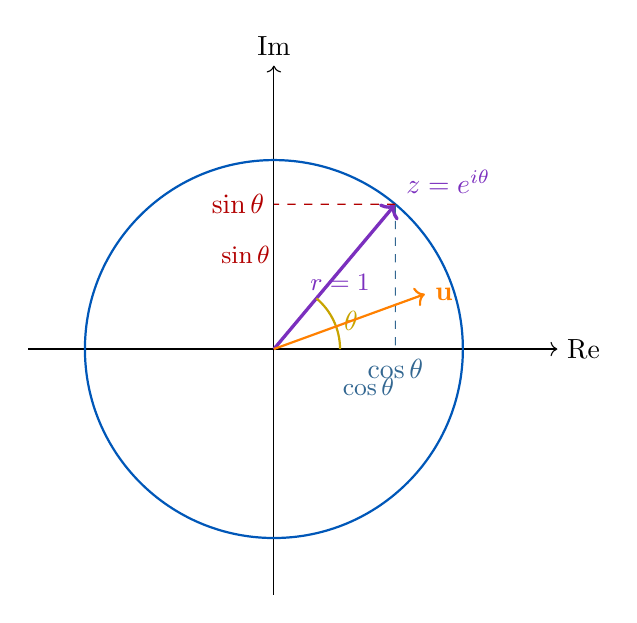
\begin{tikzpicture}[scale=2.4]
  % Axes
  \draw[->] (-1.3,0) -- (1.5,0) node[right] {$\operatorname{Re}$};
  \draw[->] (0,-1.3) -- (0,1.5) node[above] {$\operatorname{Im}$};
  % Unit circle
  \draw[thick, collibraBlue] (0,0) circle (1);
  % Vector z
  \def\ang{50}
  \coordinate (Z) at ({cos(\ang)},{sin(\ang)});
  \draw[->, very thick, quantumViolet] (0,0) -- (Z)
        node[above right] {$z = e^{i\theta}$};
  % Angle arc
  \draw[escherGold, thick] (0.35,0) arc (0:\ang:0.35)
        node[midway, right, escherGold] {$\theta$};
  % cos projection
  \draw[dashed, pgGreen] (Z) -- ({cos(\ang)},0)
        node[below, pgGreen] {$\cos\theta$};
  % sin projection
  \draw[dashed, red!70!black] (Z) -- (0,{sin(\ang)})
        node[left, red!70!black] {$\sin\theta$};
  % Second vector u
  \def\angU{20}
  \coordinate (U) at ({0.85*cos(\angU)},{0.85*sin(\angU)});
  \draw[->, thick, orange] (0,0) -- (U) node[right] {$\mathbf{u}$};
  % Angle label
  \node at (0.5,-0.2) [pgGreen] {\small $\cos\theta$};
  \node at (-0.15,0.5) [red!70!black] {\small $\sin\theta$};
  % Labels
  \node at (0.35,0.35) [quantumViolet, font=\small] {$r=1$};
\end{tikzpicture}
\end{center}

% ════════════════════════════════════════════════════════════════════════════
\section{\texttt{cosine().similarity().complex().resolve().xml().catalog().collibra()}}
% ════════════════════════════════════════════════════════════════════════════

\subsection{Cosine similarity in $\mathbb{C}^n$}

For vectors $\mathbf{u}, \mathbf{v} \in \mathbb{C}^n$:
\[
  \cossim(\mathbf{u}, \mathbf{v})
  = \frac{\operatorname{Re}\!\left(\langle\mathbf{u},\mathbf{v}\rangle\right)}{|\mathbf{u}|\,|\mathbf{v}|}
  = \frac{\operatorname{Re}\!\left(\sum_{k=1}^n \bar{u}_k v_k\right)}
         {\sqrt{\sum_k |u_k|^2}\,\sqrt{\sum_k |v_k|^2}}
  \in [-1, 1]
\]

Quantum analog: the real part of the transition amplitude:
\[
  \cossim(\ket{\psi}, \ket{\phi}) = \operatorname{Re}\!\braket{\psi}{\phi}
\]

\subsection{Angular resolution on the complex plane}

\[
  \theta(\mathbf{u},\mathbf{v})
  = \arccos\!\left(\frac{\operatorname{Re}\langle\mathbf{u},\mathbf{v}\rangle}{|\mathbf{u}||\mathbf{v}|}\right)
  \in [0, \pi]
\]

For complex exponential embeddings $\mathbf{u}_k = e^{i\phi_k}$:
\[
  \cossim = \operatorname{Re}\!\left(e^{i(\phi_v - \phi_u)}\right) = \cos(\phi_v - \phi_u)
\]

\subsection{Resolution chain to Collibra}

\[
  \texttt{cosine()} \xrightarrow{\;\cos\theta\;} \texttt{similarity()}
  \xrightarrow{\;\mathbb{C}^n\;} \texttt{complex()}
  \xrightarrow{\;\theta \to \text{IRI}\;} \texttt{resolve()}
  \xrightarrow{\;\text{DOM}\;} \texttt{xml()}
  \xrightarrow{\;\text{DCAT}\;} \texttt{catalog()}
  \xrightarrow{\;\text{REST}\;} \texttt{collibra()}
\]

Each step:
\begin{enumerate}
  \item \texttt{cosine(u,v)} — compute $\cos\theta$ in $\mathbb{C}^n$
  \item \texttt{similarity()} — threshold and rank candidates
  \item \texttt{complex()} — embed result in complex vector space
  \item \texttt{resolve()} — map angle $\theta$ to a Collibra IRI
  \item \texttt{xml()} — serialise as \texttt{chip-queries.xml} node
  \item \texttt{catalog()} — insert into DCAT catalog graph
  \item \texttt{collibra()} — POST to Collibra REST \texttt{/assets}
\end{enumerate}

% ════════════════════════════════════════════════════════════════════════════
\section{\texttt{bubbleLeader().builder().\ldots.paulGraham()}}
\label{sec:bubble}
% ════════════════════════════════════════════════════════════════════════════

\subsection{The chain as function composition}

Let $\mathcal{F}$ be the set of 13 functions. The chain is:
\[
  \Xi = \texttt{paulGraham} \circ \underbrace{\texttt{pg} \circ \texttt{pg}}_{\text{PostgreSQL} \times 2}
      \circ \texttt{escher} \circ \texttt{godel} \circ \texttt{math}
      \circ \texttt{f} \circ \texttt{c}
      \circ \texttt{clojure} \circ \texttt{groovy}
      \circ \texttt{piotr} \circ \texttt{builder} \circ \texttt{bubbleLeader}
\]

As a monad bind sequence (Haskell-style):
\[
  \Xi\, x = x \gg\!= \texttt{bubbleLeader}
              \gg\!= \texttt{builder}
              \gg\!= \texttt{piotr}
              \gg\!= \texttt{groovy}
              \gg\!= \texttt{clojure}
              \gg\!= \texttt{c}
              \gg\!= \texttt{f}
              \gg\!= \texttt{math}
              \gg\!= \texttt{godel}
              \gg\!= \texttt{escher}
              \gg\!= \texttt{pg}
              \gg\!= \texttt{pg}
              \gg\!= \texttt{paulGraham}
\]

\subsection{Layer definitions}

\begin{center}
\begin{tabular}{@{}lllp{6cm}@{}}
\toprule
\textbf{Layer} & \textbf{Domain} & \textbf{Type} & \textbf{Role in chain}\\
\midrule
\texttt{bubbleLeader}  & Architecture & Selector   & Elect the leader element; Float max to top \\
\texttt{builder}       & GoF pattern  & Factory    & Gang of Four Builder — accumulate config \\
\texttt{piotr}         & Coordination & Orchestrator & Cross-language coordination point \\
\texttt{groovy}        & JVM          & DSL        & Groovy closure / JProfiler target \\
\texttt{clojure}       & JVM          & Functional & Clojure pure-function pass; persistence core \\
\texttt{c}             & Systems      & Native     & C layer — zero-copy, cache-aligned structs \\
\texttt{f}             & Functional   & Type       & F-algebra / fixed-point functor \\
\texttt{math}          & Mathematics  & Symbolic   & Symbolic algebra (SymPy / Mathematica) \\
\texttt{godel}         & Logic        & Meta       & Gödel encoding; self-reference check \\
\texttt{escher}        & Recursion    & Fractal    & Fixed-point combinator; visual tiling \\
\texttt{pg}            & Storage      & SQL        & PostgreSQL query layer (first \texttt{pg}) \\
\texttt{pg}            & Authority    & LISP       & Paul Graham — Arc/LISP wisdom pass \\
\texttt{paulGraham}    & Philosophy   & Terminal   & Terminal evaluation: simplicity, startup \\
\bottomrule
\end{tabular}
\end{center}

\subsection{Gödel layer}

Gödel's first incompleteness theorem applied to the chain:
\[
  \forall F \text{ consistent and sufficiently expressive}:
  \exists \sigma_F \text{ s.t. } F \not\vdash \sigma_F \land F \not\vdash \neg\sigma_F
\]

Gödel numbering of chain element $f_k$:
\[
  \gonum{f_k} = \prod_{j=1}^{|\text{tokens}(f_k)|} p_j^{a_j}
\]
where $p_j$ is the $j$-th prime and $a_j$ the token code.
The chain's self-referential invariant: $\gonum{\Xi} \not\in \Xi$.

\subsection{Escher layer}

Self-reference as fixed-point combinator (Y-combinator):
\[
  Y = \lambda f . \bigl(\lambda x . f(xx)\bigr)\bigl(\lambda x . f(xx)\bigr)
\]
\[
  \texttt{escher}(f) = Y\,f = f(Y\,f) = f(f(f(\cdots)))
\]

Visually: $M.\!C.\ \text{Escher} \equiv $ ``Drawing Hands'' $\equiv$ the chain
pointing at itself through \texttt{godel} $\circ$ \texttt{escher}.

\subsection{Paul Graham layer}

The terminal evaluation reduces the chain to the LISP primitive:
\[
  \texttt{paulGraham}(e) = \text{eval}(e,\, \texttt{nil})
  \quad\text{where}\quad
  e \in \{atom, eq, car, cdr, cons, cond, lambda\}
\]

Arc's thesis: \emph{``Succinctness is power.''} Therefore:
\[
  |\Xi| \text{ should be minimal subject to } \mathcal{U}(\Xi) \text{ being maximal}
\]

% ════════════════════════════════════════════════════════════════════════════
\section{Stack $+$ Queue in Quantum Terms — Unified}
% ════════════════════════════════════════════════════════════════════════════

\subsection{Quantum register}

Combine stack $\ket{S}$ and queue $\rho_Q$ in a joint Hilbert space
$\mathcal{H}_S \otimes \mathcal{H}_Q$:
\[
  \ket{\Psi} = \ket{S} \otimes \rho_Q^{1/2}
\]

\textbf{Stack operations} act on $\mathcal{H}_S \otimes \hat{\mathbf{1}}_Q$:
\[
  \Push_S = \hat{a}^\dagger_S \otimes \hat{\mathbf{1}}_Q, \qquad
  \Pop_S  = \hat{a}_S         \otimes \hat{\mathbf{1}}_Q
\]

\textbf{Queue operations} act on $\hat{\mathbf{1}}_S \otimes \mathcal{H}_Q$:
\[
  \Enq_Q = \hat{\mathbf{1}}_S \otimes U_{\text{enq}},\qquad
  \Deq_Q = \hat{\mathbf{1}}_S \otimes \operatorname{Tr}_1
\]

\subsection{Entangled stack-queue}

When the stack and queue are entangled (e.g.\ after a \texttt{popToQueue}):
\[
  \ket{\Psi_{\text{entangled}}} = \frac{1}{\sqrt{n}}\sum_{k=0}^{n-1}
  \ket{k}_S \otimes \ket{n-1-k}_Q
\]

Measurement collapses both simultaneously.

\subsection{Quantum complexity bounds}

\begin{center}
\begin{tabular}{@{}lll@{}}
\toprule
\textbf{Operation} & \textbf{Classical} & \textbf{Quantum}\\
\midrule
Push / Enqueue      & $O(1)$             & $O(1)$ (unitary gate)\\
Pop / Dequeue       & $O(1)$             & $O(1)$ (partial trace)\\
Search              & $O(n)$             & $O(\sqrt{n})$ (Grover)\\
Sort (bubble)       & $O(n^2)$           & $O(n^{3/2})$ (quantum bubble)\\
\bottomrule
\end{tabular}
\end{center}

Quantum bubble sort uses the \texttt{bubbleLeader} comparator as a quantum oracle:
\[
  U_{\text{oracle}}\ket{i,j} = (-1)^{f(i,j)}\ket{i,j},
  \quad f(i,j) = \begin{cases}1 & a_i > a_j \\ 0 & \text{else}\end{cases}
\]

% ════════════════════════════════════════════════════════════════════════════
\section{MathML Fragment}
% ════════════════════════════════════════════════════════════════════════════

The following MathML encoding of $e^{i\pi}+1=0$ is equivalent to the
\LaTeX{} above and is used in the XML catalog node:

\begin{lstlisting}[language=XML, caption={MathML: Euler's identity}]
<math xmlns="http://www.w3.org/1998/Math/MathML">
  <mrow>
    <msup><mi>e</mi>
      <mrow><mi>i</mi><mi>&#x3C0;</mi></mrow>
    </msup>
    <mo>+</mo><mn>1</mn><mo>=</mo><mn>0</mn>
  </mrow>
</math>
\end{lstlisting}

Cosine similarity in MathML:
\begin{lstlisting}[language=XML, caption={MathML: cosine similarity}]
<math xmlns="http://www.w3.org/1998/Math/MathML">
  <mrow>
    <mi>cos_sim</mi>
    <mo>(</mo><mi mathvariant="bold">u</mi><mo>,</mo>
              <mi mathvariant="bold">v</mi><mo>)</mo>
    <mo>=</mo>
    <mfrac>
      <mrow><mi>Re</mi><mo>&#x27E8;</mo>
            <mi mathvariant="bold">u</mi><mo>,</mo>
            <mi mathvariant="bold">v</mi>
            <mo>&#x27E9;</mo></mrow>
      <mrow><mo>|</mo><mi mathvariant="bold">u</mi><mo>|</mo>
            <mo>|</mo><mi mathvariant="bold">v</mi><mo>|</mo></mrow>
    </mfrac>
  </mrow>
</math>
\end{lstlisting}

% ════════════════════════════════════════════════════════════════════════════
\section{Summary: Symbol Table}
% ════════════════════════════════════════════════════════════════════════════

\begin{multicols}{2}
\begin{tabular}{@{}ll@{}}
$\ket{\psi}$           & Quantum ket state \\
$\bra{\phi}$           & Quantum bra (dual) \\
$\hat{a},\hat{a}^\dagger$ & Pop/Push (annihilation/creation) \\
$\hat{N}$              & Number operator \\
$\rho$                 & Density matrix (queue) \\
$\operatorname{Tr}_1$  & Partial trace (dequeue) \\
$G_{\mu\nu}$           & Einstein tensor \\
$T_{\mu\nu}$           & Stress-energy (usage) \\
$\mathcal{U}$          & Ultimate metric \\
$O, \Omega, \Theta$    & Knuth asymptotics \\
\end{tabular}
\columnbreak
\begin{tabular}{@{}ll@{}}
$\uparrow\uparrow$     & Knuth up-arrow \\
$\JD(Y,M,D)$           & Julian Day Number \\
$\Ctable{AAAA\ldots FFFFF}$ & Shiva code table \\
$\Xi$                  & BubbleLeader chain \\
$\gonum{\cdot}$        & Gödel number \\
$Y$                    & Y-combinator (Escher) \\
$\cos\theta$           & Cosine similarity \\
$e^{i\theta}$          & Complex unit vector \\
$\cossim(\mathbf{u},\mathbf{v})$ & Complex cosine sim \\
$\Lambda_{\text{latency}}$ & Data cosmological const \\
\end{tabular}
\end{multicols}

\bigskip\hrule\bigskip
\noindent
\small\textcolor{godelGray}{%
  \texttt{chip-quantum-catalog.tex} $\cdot$
  Singine Collibra $\cdot$
  \texttt{cosine().similarity().complex().resolve().xml().catalog().collibra()}\\
  Grammar: \texttt{docs/xml/chip-queries.xml} $\cdot$
  Python: \texttt{singine\_collibra/quantum\_catalog.py} $\cdot$
  SVG: \texttt{docs/quantum/complex-plane.svg}
}

\end{document}
